% One harness, drawn: the C++ module (implementation M), its contract C = (A, G) on the ports,
% the monitor, and the evidence ledger E. The example is the built module rate_pid.
% Build: pdflatex single-harness-detailed.tex
\documentclass[border=8pt]{standalone}
\usepackage[T1]{fontenc}
\usepackage[default]{sourcesanspro}
\usepackage[scaled=0.95]{inconsolata}
\usepackage{amsmath,amssymb}
\usepackage{sansmath}
\usepackage{tikz}
\usetikzlibrary{arrows.meta,calc}
\definecolor{umdred}{HTML}{E21833}
\definecolor{ink}{HTML}{262626}
\definecolor{mid}{HTML}{636363}
\definecolor{pale}{HTML}{F3F3F3}
\definecolor{goldpale}{HTML}{FFF4C2}
\definecolor{golddark}{HTML}{7A5C00}
\definecolor{kw}{HTML}{FF7B72}
\definecolor{nm}{HTML}{D2A8FF}
\definecolor{tx}{HTML}{C9D1D9}
\definecolor{cm}{HTML}{8B949E}
\definecolor{ok}{HTML}{2E7D32}
\begin{document}
\sansmath
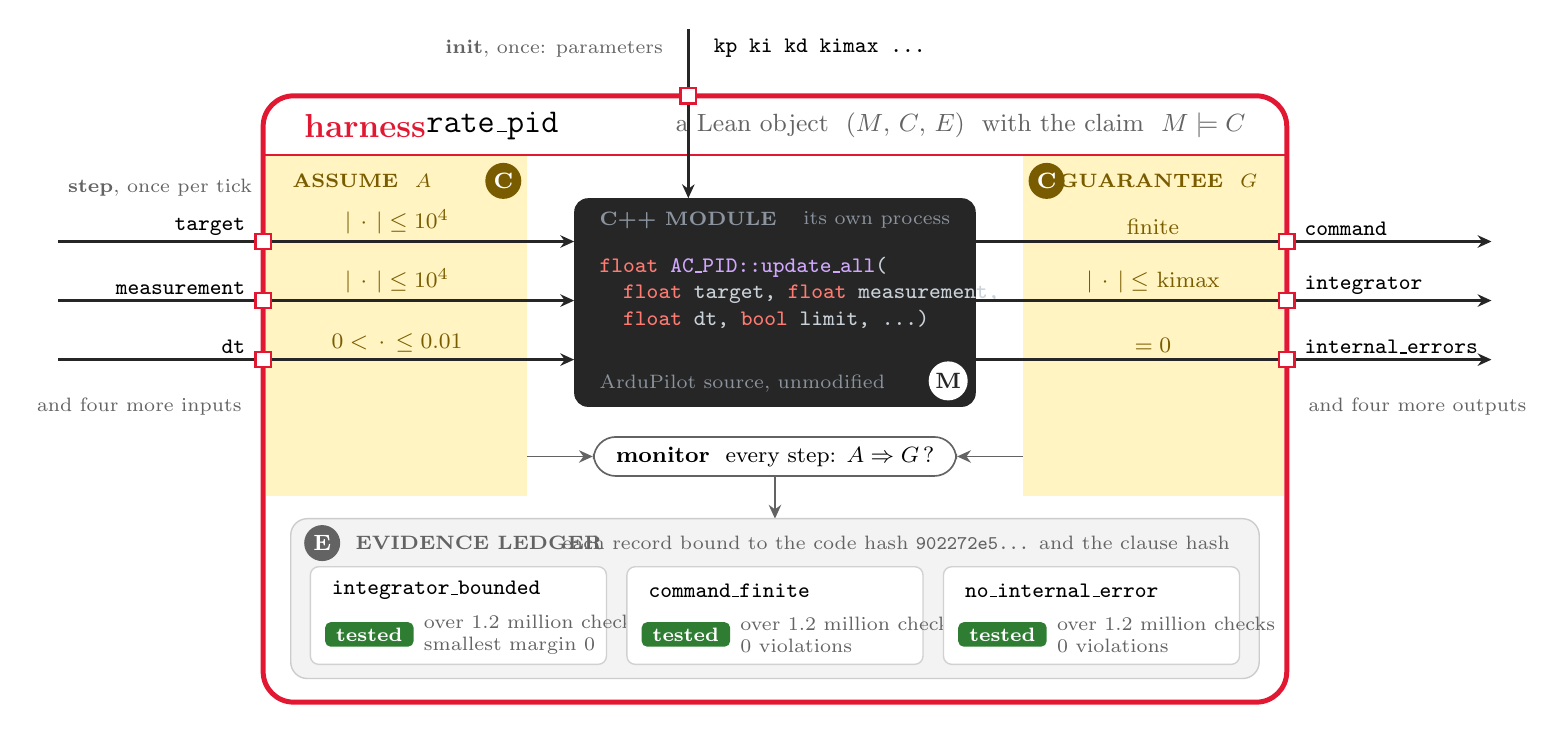
\begin{tikzpicture}[x=1cm,y=1cm,>={Stealth[length=5pt,width=4.5pt]},font=\small,
  port/.style={draw=umdred,fill=white,line width=0.9pt,minimum size=5.5pt,inner sep=0pt},
  wire/.style={line width=0.9pt,ink},
  badge/.style={circle,inner sep=1.2pt,minimum size=13pt,font=\bfseries\footnotesize,text=white},
  lbl/.style={font=\bfseries\scriptsize},
  card/.style={draw=black!18,fill=white,rounded corners=3pt,line width=0.5pt}]

% ---------------- shell
\draw[rounded corners=11pt,line width=1.8pt,umdred,fill=white] (0,0) rectangle (13,7.7);
\draw[umdred,line width=0.6pt] (0,6.95)--(13,6.95);
\node[anchor=west,font=\bfseries\large,text=umdred] at (0.4,7.32) {harness};
\node[anchor=west,font=\ttfamily\large] at (1.95,7.32) {rate\_pid};
\node[anchor=east,text=mid] at (12.6,7.32) {a Lean object \ $(M,\,C,\,E)$ \ with the claim \ $M \models C$};

% ---------------- contract strips
\fill[goldpale] (0.03,2.62) rectangle (3.35,6.93);
\fill[goldpale] (9.65,2.62) rectangle (12.97,6.93);
\node[lbl,text=golddark,anchor=west] at (0.25,6.62) {ASSUME \ $A$};
\node[lbl,text=golddark,anchor=east] at (12.75,6.62) {GUARANTEE \ $G$};
\node[badge,fill=golddark] at (3.05,6.62) {C};
\node[badge,fill=golddark] at (9.95,6.62) {C};

% ---------------- the C++ module
\fill[ink,rounded corners=5pt] (3.95,3.75) rectangle (9.05,6.4);
\node[lbl,text=cm,anchor=west] at (4.15,6.12) {C++ MODULE};
\node[font=\scriptsize,text=cm,anchor=east] at (8.85,6.12) {its own process};
\node[anchor=west,font=\ttfamily\footnotesize,text=tx,align=left] at (4.15,5.2)
  {{\color{kw}float} {\color{nm}AC\_PID::update\_all}(\\
   \ \ {\color{kw}float} target, {\color{kw}float} measurement,\\
   \ \ {\color{kw}float} dt, {\color{kw}bool} limit, ...)};
\node[font=\scriptsize,text=cm,anchor=west] at (4.15,4.05) {ArduPilot source, unmodified};
\node[badge,fill=white,text=ink] at (8.7,4.08) {M};

% ---------------- inputs
\foreach \y/\name/\cl in {5.85/target/{$|\,\cdot\,|\le 10^{4}$},5.1/measurement/{$|\,\cdot\,|\le 10^{4}$},4.35/dt/{$0<\,\cdot\,\le 0.01$}}{
  \draw[wire,->] (-2.6,\y)--(3.95,\y);
  \node[port] at (0,\y) {};
  \node[anchor=south east,font=\ttfamily\footnotesize,inner sep=2pt] at (-0.15,\y) {\name};
  \node[anchor=south,font=\footnotesize,text=golddark,inner sep=2.5pt] at (1.7,\y) {\cl};
}
\node[font=\scriptsize,text=mid,anchor=east] at (-0.15,3.75) {and four more inputs};
\node[font=\scriptsize,text=mid,anchor=south west] at (-2.6,6.3) {\textbf{step}, once per tick};

% ---------------- outputs
\foreach \y/\name/\cl in {5.85/command/{finite},5.1/integrator/{$|\,\cdot\,|\le$ kimax},4.35/internal\_errors/{$=0$}}{
  \draw[wire,->] (9.05,\y)--(15.6,\y);
  \node[port] at (13,\y) {};
  \node[anchor=south west,font=\ttfamily\footnotesize,inner sep=2pt] at (13.15,\y) {\name};
  \node[anchor=south,font=\footnotesize,text=golddark,inner sep=2.5pt] at (11.3,\y) {\cl};
}
\node[font=\scriptsize,text=mid,anchor=west] at (13.15,3.75) {and four more outputs};

% ---------------- parameters
\draw[wire,->] (5.4,8.55)--(5.4,6.4);
\node[port] at (5.4,7.7) {};
\node[anchor=west,font=\ttfamily\footnotesize] at (5.6,8.3) {kp ki kd kimax ...};
\node[anchor=east,font=\scriptsize,text=mid] at (5.2,8.3) {\textbf{init}, once: parameters};

% ---------------- monitor
\node[draw=mid,fill=white,rounded corners=8pt,line width=0.6pt,inner xsep=8pt,inner ysep=3.5pt,
      font=\footnotesize] (mon) at (6.5,3.12) {\textbf{monitor}\ \ every step: $A \Rightarrow G$\,?};
\draw[mid,line width=0.6pt,->] (3.35,3.12)--(mon.west);
\draw[mid,line width=0.6pt,->] (9.65,3.12)--(mon.east);
\draw[mid,line width=0.6pt,->] (mon.south)--(6.5,2.33);

% ---------------- evidence ledger
\draw[black!20,fill=pale,rounded corners=6pt,line width=0.5pt] (0.35,0.3) rectangle (12.65,2.33);
\node[badge,fill=mid] at (0.75,2.02) {E};
\node[lbl,text=mid,anchor=west] at (1.05,2.02) {EVIDENCE LEDGER};
\node[font=\scriptsize,text=mid,anchor=east] at (12.4,2.02)
  {each record bound to the code hash {\ttfamily 902272e5...} and the clause hash};
\foreach \x/\name/\res in {0.6/integrator\_bounded/{smallest margin 0},4.62/command\_finite/{0 violations},8.64/no\_internal\_error/{0 violations}}{
  \draw[card] (\x,0.48) rectangle (\x+3.76,1.72);
  \node[anchor=west,font=\ttfamily\footnotesize] at (\x+0.15,1.42) {\name};
  \node[anchor=west,fill=ok,text=white,rounded corners=2pt,font=\bfseries\scriptsize,inner xsep=4pt,
        inner ysep=2pt] (k) at (\x+0.18,0.86) {tested};
  \node[anchor=west,font=\scriptsize,text=mid,align=left] at (k.east) {over 1.2 million checks\\\res};
}
\end{tikzpicture}
\end{document}
